%% 30-resource.tex — Resource Description

\section{Resource Description}
\label{sec:resource}

GEMEA (/ɡəˈmeɪ.jə/) is a knowledge graph over approximately 26.8 million objects from the German Digital Library (DDB), organized into named graphs in QLever and served through SHMARQL\footnote{\url{https://gemea.ise.fiz-karlsruhe.de/shmarql/}} as a SPARQL endpoint and Linked Data browser; the dataset is available for download at \url{https://gemea.ise.fiz-karlsruhe.de/downloads}, and the MCP/MCPO integration is released as self-hosting setup scripts.

\subsection{GEMEA}
\label{sec:resource:kg}

The source data is the digitised proportion of the DDB corpus: the DDB aggregates metadata records from more than 500 German cultural heritage institutions across 7 sectors (\textit{Bibliothek}, \textit{Archiv}, \textit{Museum}, \textit{Mediathek}, \textit{Denkmal}, \textit{Forschung}, \textit{Sonstiges}), many of which describe objects that have not been scanned, photographed, or recorded; GEMEA covers only those records for which a digital surrogate exists.

DDB JSON-LD records are converted to N-Quads by a custom transformation pipeline that maps EDM predicates to RDA and mocho (Section~\ref{sec:resource:mocho}) properties and partitions output into named graphs by content layer.
A post-processing phase links literary and musical works to GND authority records through several passes employing NLP models, adding work-level links to a fourth named graph.
The QLever index is organised as four named graphs: \texttt{graph/ddbedm} (verbatim EDM passthrough), \texttt{graph/mocho} (mocho-aligned triples), \texttt{graph/prov} (PROV-O provenance), and \texttt{graph/work} (GND work links), allowing queries to target a single content layer without full-corpus scans.

\paragraph{Scale.}
Table~\ref{tab:scale} reports object and triple counts per sector and named graph.
Digitised DDB objects are retrieved by querying the DDB Search API\footnote{\url{https://api.deutsche-digitale-bibliothek.de/2/search}}, filtering for digitized objects only (\texttt{digitalisat:true}); JSON records are fetched per object from the DDB Items API.\footnote{\url{https://api.deutsche-digitale-bibliothek.de/2/items}}
During serialisation to RDF triples, malformed IRIs are percent-encoded to produce valid IRI references, and internal DDB identifiers are replaced with \texttt{urn:} URNs to ensure global uniqueness of entity URIs across the graph.
Rights are not uniform and are queryable directly via \texttt{dcterms:rights}; see Section~\ref{sec:quality:limitations}.

\begin{table}[h]
\centering
\caption{Object and triple counts per sector.}
\label{tab:scale}
\begin{tabular}{|l|r|r|r|r|r|}
\hline
\multicolumn{1}{|c|}{\multirow{2}{*}{\textbf{Sector}}} & \multicolumn{1}{c|}{\multirow{2}{*}{\textbf{Objects}}} & \multicolumn{1}{c|}{\multirow{2}{*}{\textbf{Total triples}}} & \multicolumn{3}{c|}{\textbf{Named graph triples}} \\
\cline{4-6}
 & & & \textbf{DDB-EDM} & \textbf{MOCHO} & \textbf{PROV} \\
\hline
\rowcolor{gray!15}
Library           & 18,338,116 & 1,930,178,220 & 1,040,390,087 & 356,952,292 & 532,835,841 \\
\hline
Archive           &  3,456,119 & 467,439,123 & 259,483,277 & 61,795,115 & 146,160,731 \\
\hline
\rowcolor{gray!15}
Museum            &  2,011,841 & 230,484,127 & 123,795,378 & 48,164,578 & 58,524,171 \\
\hline
Media Library     &  1,709,846 & 258,176,923 & 145,905,243 & 58,871,240 & 53,400,440 \\
\hline
\rowcolor{gray!15}
Research          &  1,165,891 & 138,118,201 & 75,842,237 & 24,633,128 & 37,642,836 \\
\hline
Monument Preserv. &     79,393 & 9,020,751 & 4,852,432 & 1,555,297 & 2,613,022 \\
\hline
\rowcolor{gray!15}
Others            &     85,408 & 9,996,438 & 5,487,618 & 1,958,508 & 2,550,312 \\
\hline
\rowcolor{gray!30}
\textbf{Total}    & \textbf{26,846,614} & \textbf{3,043,413,783} & \textbf{1,655,756,272} & \textbf{553,930,158} & \textbf{833,727,353} \\
\hline
\end{tabular}
\end{table}

\subsection{MOCHO Alignment}
\label{sec:resource:mocho}

EDM is designed for cross-institutional aggregation: all objects share a flat \texttt{edm:ProvidedCHO} type, DC/EDM predicates carry no WEMI-level distinction, and agent roles are untyped, making work-level grouping, typed predicate queries, and structured semantic querying over the collection dependent on further alignment.
The \textbf{MOCHO} ontology~\cite{tan2026navigating} addresses this by assigning domain- and mediatype-specific types to ProvidedCHOs, routing EDM predicates to typed properties at the correct WEMI level, and grouping co-manifesting records into \texttt{mocho:Work} entities where GND authority links are available.
The alignment is developed and validated on the \textit{Goethe-Faust corpus} (115,432 records), which serves as the reference implementation corpus before scaling to the full 26.8M-object DDB collection.
The full alignment table and per-class statistics are released in the GEMEA GitHub repository.\footnote{\url{https://github.com/anntanp/gemea/tree/develop}}

\paragraph{Corpus-driven class dispatch.}
A key finding from corpus analysis is that DDB-EDM property semantics are sector-dependent and not declared in the schema: \texttt{dc:type} carries a mixture of free-text terms and controlled-vocabulary in library records, free-text strings in museum records, and structural hierarchy codes in archive records; \texttt{ddb:hierarchyType} (htype) is present in archive and library strata but mostly absent in  non-\textt{TEXT} media types across museum, media library, and monument sectors entirely.
These differences surface only through corpus measurement.
Signal coverage is therefore quantified per sector~$\times$~mediatype stratum before any dispatch logic is implemented: Archive text records carry both htype and dc:type in 99.6\% of cases; Library text records are htype-only in 31\%; Museum, Media Library, and Monument records carry no htype at all.
This coverage profile sets dispatch priority per stratum: htype-first for Archive and Library, dc:type-first for the remaining sectors, rather than a uniform fallback chain.
Scope boundaries where real EDM encodings deviate from the alignment assumptions are documented in Section~\ref{sec:quality}.

\paragraph{Iterative ontology extension.}
The target ontology is not fixed before transformation begins; instead, corpus analysis drives its extension.
Entity types encountered during inspection of the Goethe-Faust corpus (digitised photographs, cartographic objects, immovable cultural monuments) had no adequate representation in MOCHO before the alignment work.
New classes (\texttt{mocho:ImageWork}, \texttt{mocho:ImmovableWork}, \texttt{mocho:ImageObject}) are introduced in direct response to patterns surfaced in the corpus: a gap is identified, a class is defined in the ontology, alignment rules are updated, and the transform is re-run.
This cycle repeats until alignment coverage is stable across all strata.

\paragraph{Property mapping.}
Because DDB-EDM properties are DC\footnote{Dublin Core Elements (\texttt{dc:}), \url{http://purl.org/dc/elements/1.1/}}/DCT\footnote{DCMI Metadata Terms (\texttt{dcterms:}), \url{http://purl.org/dc/terms/}}-based, the RDA Registry DC-to-RDA mapping\footnote{\url{https://www.rdaregistry.info/Maps/mapRDA2DCT.html}} provides the systematic bridge to typed RDA predicates at the correct WEMI level.
RDA serves as the alignment pivot: each assigned class branches to its native domain ontology (general metadata for library records, VRA Core for visual objects, RiC-O for archival materials, Music Ontology for audio), without requiring separate DC-to-domain mappings per ontology.
Target predicates are resolved per \texttt{(target\_class, ddb-edm\_prop)} pair, with corpus inspection correcting derivation errors in the machine-generated alignment table and resolving predicate choices where the table produces spurious candidates.
For contributor roles, the LIDO event type of the \texttt{edm:Event} node linked to the \texttt{edm:ProvidedCHO} determines the emitted property (author, photographer, publisher), exploiting the event-centric aspect of EDM to capture typed role semantics invisible at the DC level.

\subsection{SHMARQL Linked Data Interface}
\label{sec:resource:shmarql}

SHMARQL~\cite{shmarql} is a lightweight Linked Data publishing layer deployed as a Docker container (\texttt{ghcr.io/epoz/shmarql}).
Entity URIs are dereferenceable, RDF is served with content negotiation (HTML, Turtle, JSON-LD), and a built-in SPARQL query editor is included.
As a SPARQL~1.1-endpoint-agnostic browser, SHMARQL is redeployable without modification and serves as the primary dereferencing interface for entity URIs minted as \texttt{urn:} identifiers for global uniqueness, which carry no native HTTP resolution.

For GEMEA, SHMARQL is deployed as a proxy over the QLever endpoint.
The deployment was validated on the Goethe-Faust corpus before scaling to GEMEA.
The GEMEA SHMARQL instance is available at \url{https://gemea.ise.fiz-karlsruhe.de/shmarql}.

\begin{figure}[H]
  \centering
  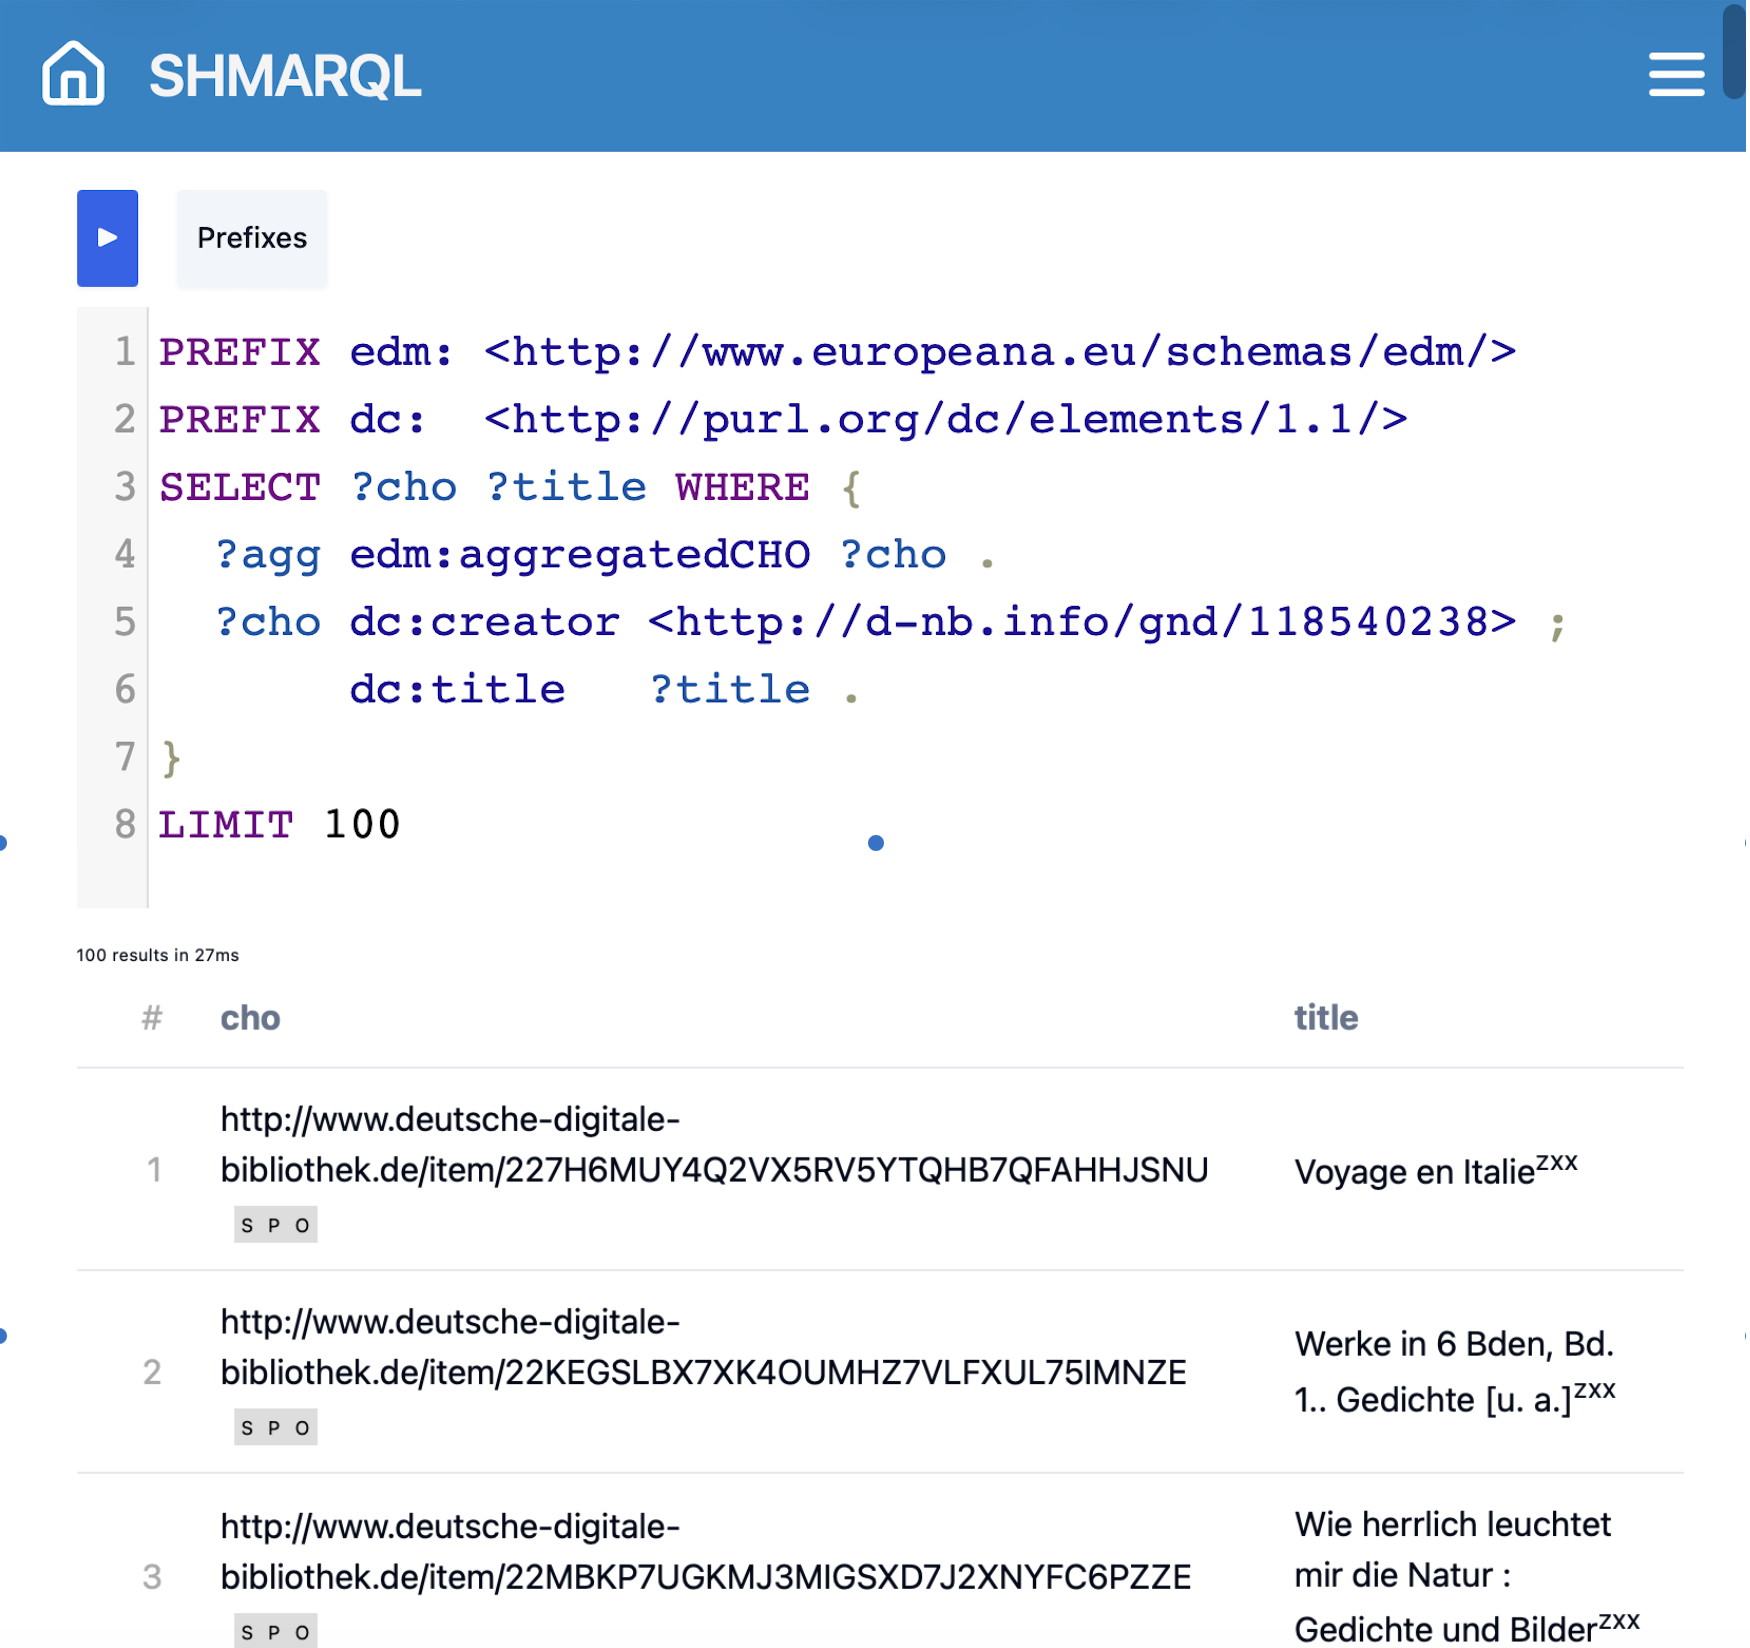
\includegraphics[width=\columnwidth]{images/shmarql-screenshot}
  \caption{SHMARQL interface showing the SPARQL query editor and entity view. The \texttt{[S]}, \texttt{[P]}, and \texttt{[O]} controls under each entity in the CHO column load all triples where that entity appears as subject, predicate, or object, enabling step-by-step graph traversal without writing SPARQL.}
  \label{fig:shmarql}
\end{figure}

\subsection{MCP/MCPO Agentic Access Layer}
\label{sec:resource:mcp}

The Model Context Protocol (MCP)~\footnote{MCP, \url{https://modelcontextprotocol.io/docs/getting-started/intro}} is an open standard for exposing tools and data sources to AI agents.
\texttt{mcp-server-qlever}~\cite{mcpqlever} is a third-party MCP server tailored for the QLever engine, exposing SPARQL query execution, schema exploration, entity search, and QLever-specific capabilities (context-sensitive autocompletion, spatial queries, query plan analysis) as MCP tools.
GEMEA's QLever endpoint is registered with \texttt{mcp-server-qlever}, making the KG queryable by any MCP-compatible agent or LLM client without custom integration code.
An MCPO~\footnote{MCPO, \url{https://github.com/open-webui/mcpo}} wrapper is also provided, exposing the endpoint as an OpenAPI-compatible HTTP interface for REST-native clients; invocation support depends on the client framework.

Setup scripts for the full stack, including MCP registration, are provided in the GEMEA GitHub repository.\footnote{\url{https://github.com/anntanp/gemea/}}

\paragraph{Example agent interaction.}
An agent is asked: \textit{``How many objects in the dataset are attributed to Goethe? Which institutions hold the most of them?''}
The agent resolves Goethe's GND identifier (\texttt{gnd:118540238}), issues a \texttt{dc:creator} query, and groups results by \texttt{edm:dataProvider}:

\begin{figure}[h]
  \begin{minipage}[t]{0.46\linewidth}
    \vspace{0pt}
    \begin{lstlisting}[language=SPARQL, basicstyle=\ttfamily\footnotesize, breaklines=true]
PREFIX dc:  <http://purl.org/dc/elements/1.1/>
PREFIX edm: <http://www.europeana.eu/schemas/edm/>
SELECT ?provider
       (COUNT(DISTINCT ?cho) AS ?n)
WHERE {
  ?cho dc:creator
    <http://d-nb.info/gnd/118540238> .
  ?agg edm:aggregatedCHO ?cho ;
       edm:dataProvider ?provider .
  FILTER(isLiteral(?provider))
}
GROUP BY ?provider
ORDER BY DESC(?n)
    \end{lstlisting}
  \end{minipage}
  \hfill
  \begin{minipage}[t]{0.50\linewidth}
    \vspace{0pt}
    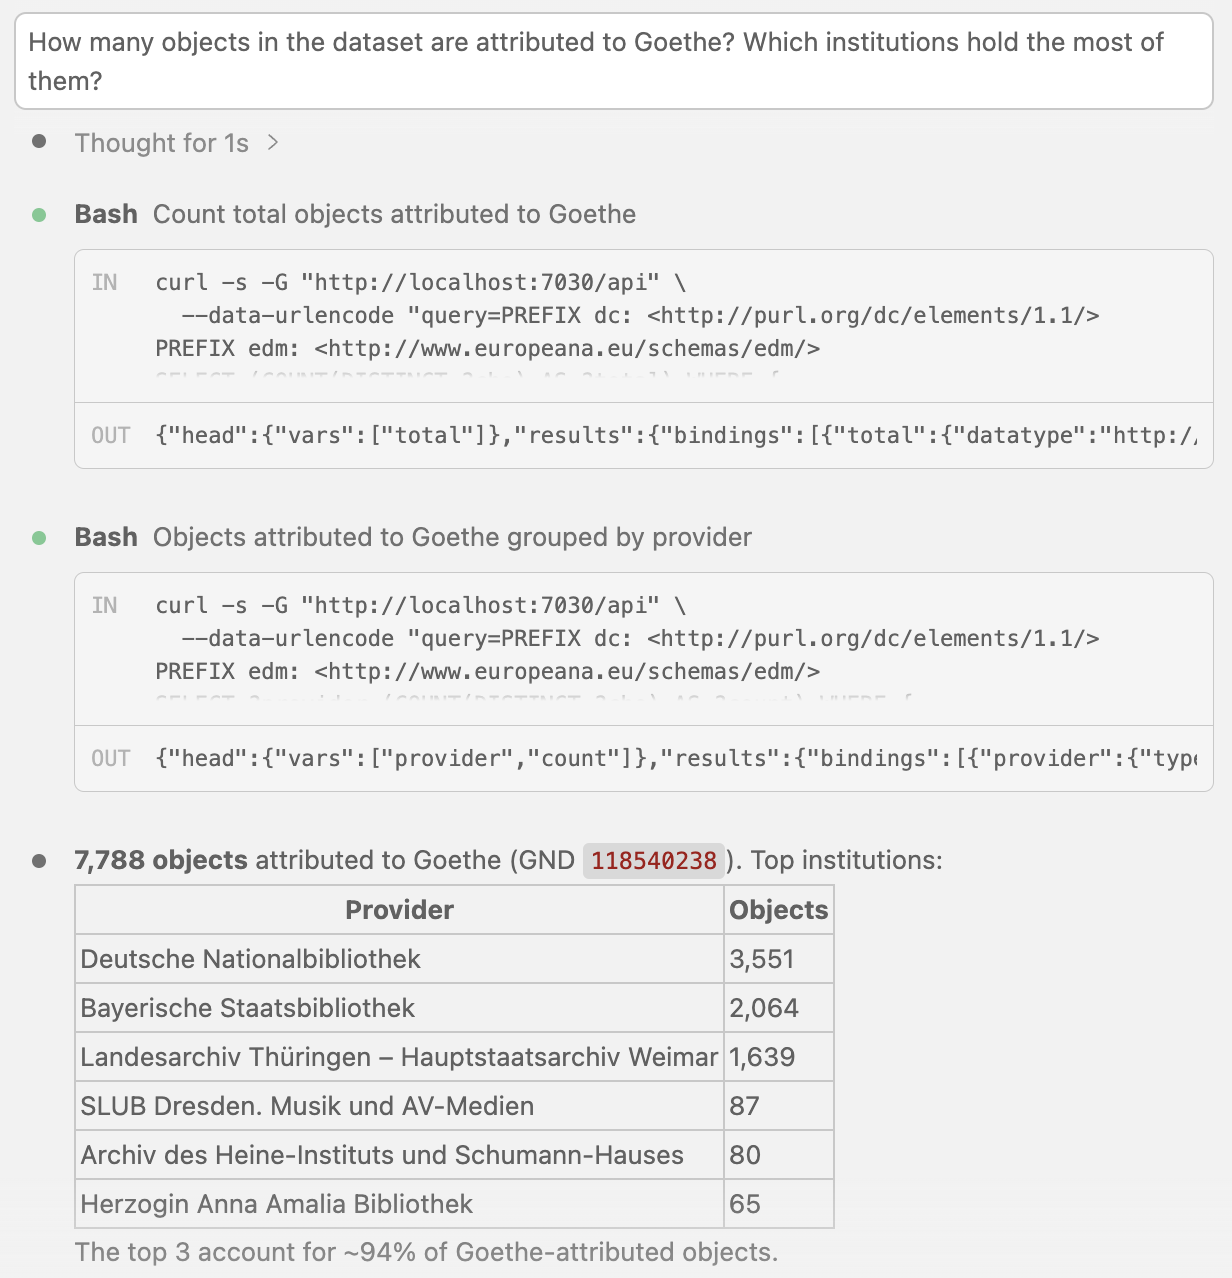
\includegraphics[width=\linewidth]{images/claude-screenshot.png}
  \end{minipage}
  \caption[SPARQL query (left) and Claude MCP session (right).]{SPARQL query issued by the agent (left) and the Claude Code MCP session (right). The query returns 7{,}788 objects across 10 institutions; the three largest holders are the Deutsche Nationalbibliothek (3{,}551), Bayerische Staatsbibliothek (2{,}064), and Landesarchiv Thüringen -- Hauptstaatsarchiv Weimar (1{,}639).\protect\footnotemark}
  \label{fig:claude-mcp}
\end{figure}
\footnotetext{Demo run on the Goethe-Faust reference corpus~\cite{goethefaust}.}
